\documentclass[a4paper]{article}

\usepackage[utf8]{inputenc}
\usepackage[T1]{fontenc}
\usepackage{natbib}
\usepackage{graphicx}
\graphicspath{{./images/}}

\begin{document}

\title{Automated analysis and planning of online marketing campaigns}
\author{Erik Brännström\\
  Chalmers University of Technology}
\date{}
\maketitle

\section{Introduction}
Duego was founded in 2010 with the idea of creating a social networking site whose target group is those who wish to meet new
people. This stands in contrast to the existing networks that either manage people who the user already knows (e.g. Facebook)
or where the user tries to find a life partner (i.e. dating sites). Online advertisement is leveraged as a way to promote the
site to new users. This is done both using targeted ads that are adapted based on the target demographics on social networks,
as well as more conventional ads on websites. Today, managing these campaigns is a manual process that is outsourced to
another company.

The wish of Duego is to automate this process using software. Such a system would be required to analyze the existing campaigns
with regard to ads and target groups along with campaign metrics such as clicks per impression, conversion ratio, etcetera, and
use this data to suggest, or even automatically add, new campaign ads. The data set that will be used in production consists of
hundreds of different campaigns, each with a large number of ads. Along with the attributes of both campaigns and ads, this means
that the complete advertisement data set consists of hundreds of thousands of attributes to be analyzed.

\section{Marketing terminology}
A number of marketing terms will be used throughout this paper. A \emph{marketing campaign}, or simply a \emph{campaign},
is comprised of one or more advertising messages, \emph{ads}, that are directed to one defined audience, the \emph{target} or 
\emph{target group}. Any ad, and by extension campaign, have numeric measures of success called \emph{metrics}. The most commonly
used are \emph{impressions}, which is the number of times an ad has been shown, and \emph{clicks}. Ads are limited to include a 
title, a body text and/or an image, as well as the mandatory URL that a user who clicks the ad will be redirected to. A target
is defined by demographic data such as age, gender, location or, in the case of for example search engine advertisement, search
terms.

\begin{figure}[htb]
\centering
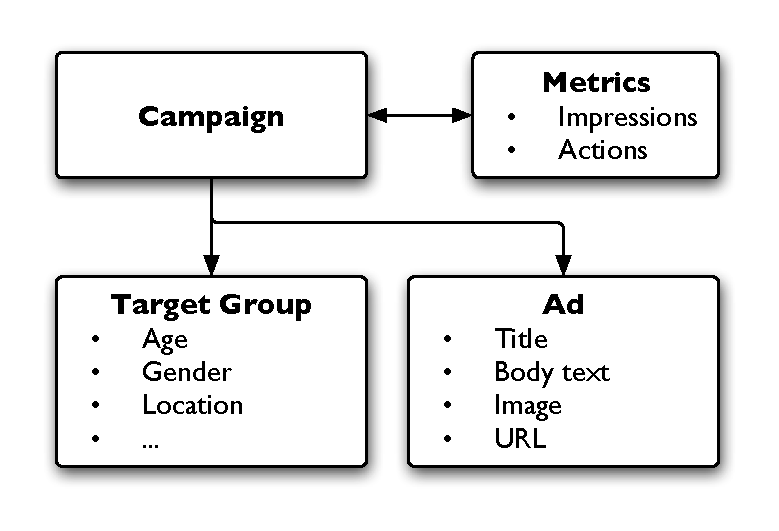
\includegraphics[width=0.7\textwidth]{campaign-terminology.eps}
\caption{Marketing terminology}
\label{fig:MarketingTerminology}
\end{figure}

As the word user is typically used to refer to a person interacting with the web site that is being marketed, we will use the word
\emph{operator} when discussing a person interacting with the system that is described in this paper to avoid confusion.

\section{Problem}
This problem statement is described from the view of Duego, however it can be generalized into a broader problem in the sphere of
software engineering, namely knowledge discovery in databases (KDD) or more specifically data mining. Data mining is the process
of delegating and automating the task of identifying useful knowledge in a large set of data to a computer, either fully or
partially. The somewhat philosophical discussion of what knowledge really is and how to define what is useful knowledge will not,
however, be covered in this paper.

\begin{figure}[htb]
\centering
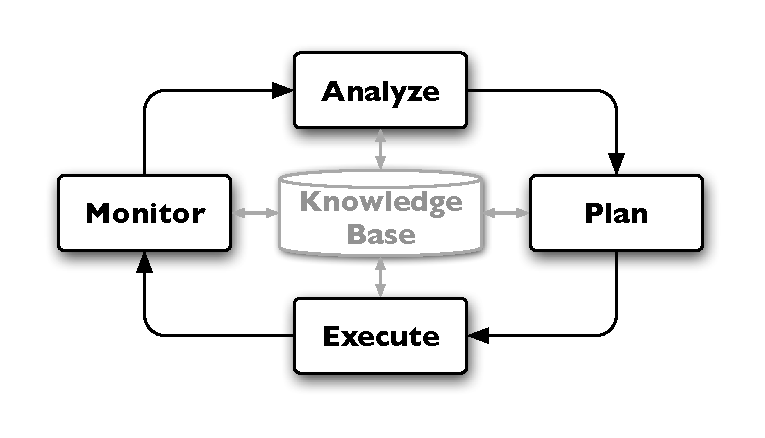
\includegraphics[width=0.7\textwidth]{mape.eps}
\caption{General MAPE control loop}
\label{fig:MAPE}
\end{figure}

Useful terminology is defined by \citet{IBM2006} in the field of autonomic computing. Figure \ref{fig:MAPE} shows an autonomic
manager, which is a component that collects data from a system and, based on this data, performs actions with the purpose of
improving the system. This control loop is divided into four sub-tasks called monitor (collect system information), analyze
(correlate and model data), plan (design behaviour required to reach goal) and execute (run the planned actions), sometimes
refered to as MAPE.

In online marketing, monitoring is the collection of metrics for online advertisement. To optimize these metrics, the gathered
information is analyzed and this analysis forms the basis for the planning of future campaigns. Once the plans are completed, the
new campaign can be launched, with new metrics being gathered and so on.

To formalize the marketing terminology described previously, a target group is an m-tuple \(T = (t_1, t_2, ..., t_m)\) and an ad is an n-tuple \(A = (a_1, a_2, ..., a_n)\). A campaign can thus be described as the pair \(C = (T, A)\) or, by flattening, \(C' = (t_1, t_2, ..., t_m, a_1, a_2, ..., a_n)\). \(C'\) will typically be the format that the system expects input.

\begin{figure}[h!]
\centering
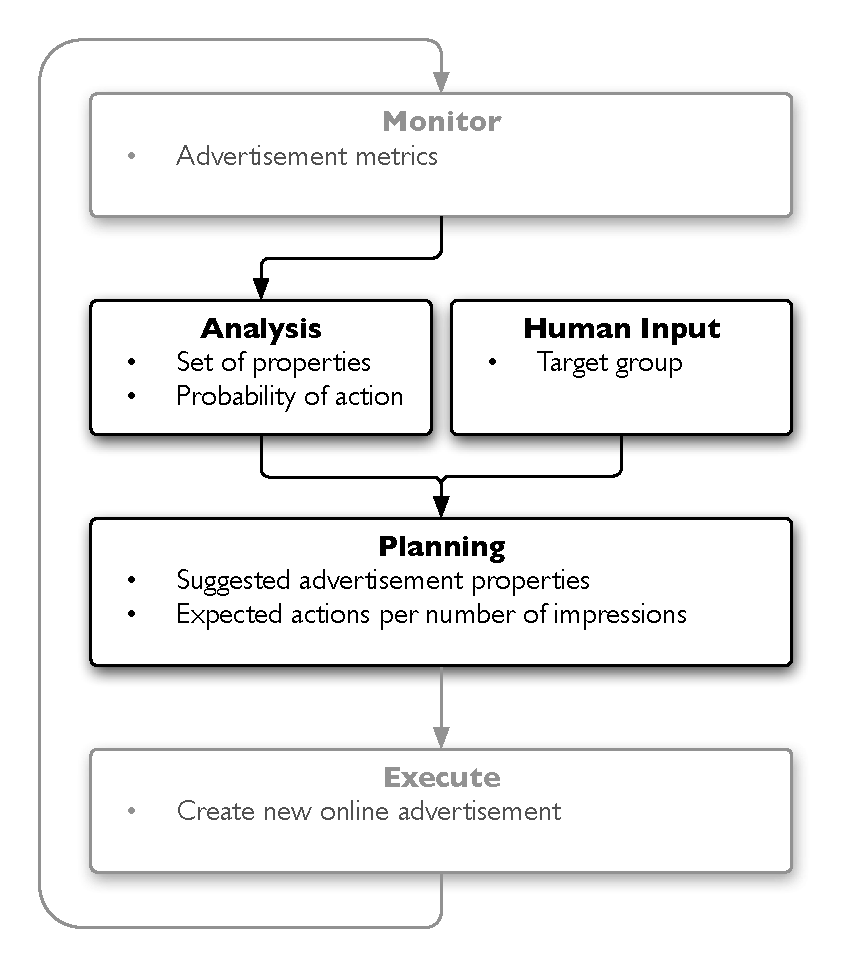
\includegraphics[width=0.7\textwidth]{mape-marketing.eps}
\caption{Online marketing automation system in control loop}
\label{fig:MAPEMarketing}
\end{figure}

Today only the monitoring is automated, where as the other parts of the process are performed manually. It is infeasible to fully
automate the whole process, due to for example the creative side of advertisement and the complex factors that decide which groups
an upcoming campaign should target. There are however certain areas that can be automated and this paper will focus on automated
analysis and planning of online marketing campaigns, shown in Figure \ref{fig:MAPEMarketing}.

A system to automate this process would require monitored data as input, which in this context equals historical data of campaigns
and their metrics as mentioned previously. This data would then be mined to identify subsets of campaign properties that are
associated with a probability that an impression of that an ad with these properties leads to an action being taken by the user.
Human input is required to specify which target group the next campaign will be aimed at, and based on this the system will
generate suggested ad properties that optimize the number of expected actions taken per impression.

\section{Scope}
Using the MAPE framework in Figure \ref{fig:MAPE}, only the analysis and planning tasks are considered part of this paper, where
as monitoring and execution are out of scope. The latter two are however relevant in the verification step, but will not be
covered as a research topic. In this context, this means for example that the feature of integrating this system with marketing
services to automatically add new ads and campaigns will not be a part of the final system.

Furthermore, the data set includes attributes whose values are free text and images. Text mining and image recognition are beyond
the scope of this project. Instead these attributes will be manually categorized, so that the value space is discrete and finite.

\section{Foundations}
A number of high-level descriptions of frameworks for knowledge discovery in databases exist \citep{Fayyad1996, Frawley1992}
and they exhibit a number of commonalities. These include the importance of having a knowledgeble human operator guiding the
process in terms of supplying domain knowledge to the system formulating the goal of the knowledge discovery; feeding discovered
knowledge back into the system; and the identification and application of a discovery method, or more specifically the data mining
algorithm(s).

In data mining, the input to a system can be described using the terms \emph{concepts}, \emph{instances} and \emph{attributes},
where concept is the actual result of the mining, i.e. what we want to be learned; an instance is one single example of data to be
mined and can be compared to a row in a database; and attribute is a property of an instance, which in the database analogy would
be a column \citep{Witten2011}.

The Weka Project has defined an input format to be used for their open source data mining software called ARFF (Attribute-Relation
File Format) \citep{Garner1995, Witten2011}. This format is used by the Weka software package, but is well-defined and can be used
as the input format for custom systems as well. \citet{Witten2011} also describe how to use implementations of Weka in custom
software projects as well as how to extend the system with new functionality.

In a highly influential paper, \citet{Quinlan1986} decribe how decision trees can be created from a training set and how well it
handles the problem of unknown attributes values and noisy data. A related paper, \citet{Quinlan1987}, deal with how generated
decision trees can be simplified in order to more easily be applied. Four different methods are evaluated, one of which is the
reformulation of the tree as a set of production rules. This specific topic is further analyzed in \citet{Quinlan1987b} where such
production rules are shown to be more compact and also in many cases improve the classification of unseen data. An added positive
effect is that production rules from separate classifications can be merged more efficiently than their original decision trees.

Standard decision trees give a best-effort boolean classification of the input data, however sometimes it might be more
appropriate to give the probability that the input belongs to each of the available classes. This can be described using
probability estimation trees (PETs). \citet{Provost2003} discuss the problems of estimating these probabilities from ordinary
decision trees and goes on to show how to increase the accuracy of the estimates by performing tree pruning more conservately and
by applying the Laplace correction.  They also show that probability-bagging, meaning the combination of results from multiple
classifiers instead of just the one, greatly improves the estimates. The suggested algorithm, called C4.4, is part of a
comparative study of PETs by \citet{Chu2011} and is shown to have an impressive accuracy, though other algorithms may still be
more appropriate. A likely candidate algorithm for this thesis is the Naive Bayes tree, which is a standard decision tree with the
difference that the leaves are Naive Bayes classifiers, providing probabilities that an instance belong to each of the available
classes.

A thorough literature study on domain-specific languages is covered by \citet{Deursen2000} and covers high-level topics, such as
potential benefits and risks of using DSLs and exemplifying with a number of languages from different areas. The article also
mentions the phases of development in the creation of a new DSL, a topic which is described in more detail by \citet{Mernik2005}.
The latter article also provides insight into the relevant choices that need be made in the creation process, and both articles
help define a useful terminology for discussing the topic of domain-specific languages.

\section{Related works}
\citet{Chen1996} give an overview of the field of data mining where they mention the aspect of multi-level data mining, which
states that correlations may not commonly exist on the lowest level of granularity, but instead by forming groups of related
items. An example given would be that a specific brand of milk does not necessarily imply the purchase of a specific brand of
bread, however purchasing milk of any kind may still be correlated to the purchase of bread irrespective of brand.

A related area in data mining is association rule learning. \citet{Agrawal1993} describe how, given a large set of
transactions containing any number of different items, rules can be identified between these items. In the case of commerce,
such rules would describe how the purchase of one product would, with a probability above a certain threshold, also infer
the purchase of another product. This method could be applicable to the problem in this paper, even though it is more of a
classification problem, and some of the necessary extensions of the method are mentioned below.

\citet{Srikant1997} expands the above research by applying contraints on the items in the resulting association rules. These
constraints can either be expressed using specific items or with taxonomy rules, e.g. if an item is a descendant or ancestor
of another item. For this problem, the relation between target groups and ads can, based on existing metrics, be restructured into
a transactional table where each transaction is an impression (in the case of the impression per click metrics) so that each entry
would have an attribute stating whether or not the impression yielded a click. The item constraint would then be used to only
formulate association rules that lead to clicks.

Considering that the original market basket problem assumes binary attributes and that relational data can contain both
quantative and categorical data, \citep{Srikant1996} gives a useful description on how such values can be mapped onto the
binary (or boolean) problem space.

\citet{Hahsler2007} presents a package for the R software environment used in statistical computing, which implements a base
for transaction databases as well as integration with two of the most common mining algorithms, Apriori and Eclat. One of the
useful implementation choices is the implementation of the sparse matrix data structure, which greatly reduces memory load.

\citet{Richardson2007} describe a model for predicting the click-through rates of ads given a set of properties in the context
of search engine advertisement. Though it is a relevant subject, the major difference between such advertisement and that which
occurs on social networking sites is targeting. Search engines uses keyword matching to select possible ads, i.e. what the user is
interested in at this moment, where as social networks can uitilize knowledge about who the user is.

\section{Solution}
The solution has been divided into one section each for the two subtasks identified in the problem description. Analysis covers
the problem of creating an appropriate model of the available data that can be used in the next stage. Planning, in turn, is the
utilization of that model with the purpose of outputting useful information to the operator.

\subsection{Analysis}
The natural distribution of the input data is very uneven because the number of impressions required to receive a click is high.
Consider the scenario of a click-through rate (CTR) of 1\%, which means that for every 100 impressions there would on average be one
click. The simplest possible classification rule would be a rule that for every instance gives the classification of no click, and
this would yield an accuracy of 99\%. Even though this is indeed an impressive number, it is of no use to us since it says nothing
about the instances that actually would yield clicks. This is refered to as the problem of imbalanced data sets as described by
\citet{Chawla2004}.

One way to deal with this problem is to increase the number of instances that we are interested in (positive instances) or
decreasing the number of negative instances in so that the total distribution is even. This is called over-sampling and under-
sampling respectively, and will remove the possibility for a classifier to simply disregard the positive instances in the
classification \citep{Chawla2004, Japkowicz2002}.

A better alternative is to use the concept of cost modification, i.e. instruct the algorithm that it is more costly to misclassify
positive instances as negative instances than vice versa, which has been shown to be as effective as over-sampling but with
increased efficiency \citep{Chawla2004, Japkowicz2002} due to the fact that it does not increase the number of instances in the
data set.

Once the monitored data has been passed to the system it will be added to the knowledge base. The data will also be used to 
generate a new analysis model of the full data set which also will be stored in the knowledge base, making it available for the
planning subsystem.

As part of the generation of an analysis model, stored estimations may be compared to the monitored data and based on their
differences the system can update a number of paramaters for the generation algorithm so that future estimates are improved.

\subsubsection{Model generation}
The model can be built by any data mining classifier algorithm that adheres to the basic requirements of handling both numerical 
and categorical values as well as generating either a decision tree or a set of decision rules, for example the PART algorithm 
\citep{Frank1998}.

To increase accuracy, a stratified tenfold cross-validation approach is recommended, which can optionally be repeated ten times to
further improve the result with an additional cost in computing time. The validation step should calculate the success rate
of the classification for each rule or leaf on each pass and average the values on completion. Confidence intervals can be
calculated using tables for the Bernoulli distribution \citep[chap. 5]{Witten2011} based on the observed success rate \(S\) and the 
number of instances that matched the rule \(N\). The probability of success is \(\rho \pm z\) with confidence \(c\).

\subsubsection{TBR - Click probability}
Once the appropriate cost matrix has been applied, the PART algorithm \citep{Frank1998} is used to mine the data for rules.
For each rule in the result, the number of instances in the data set that are covered by the rule (\(I\)) as well as how many of
those instances that are misclassified (\(M\)) is calculated. The weight added to the positive instances is refered to as \(W\).
Using these known values, an expected probability of the rule producing a click, \(\rho\), can be calculated.

\[
	\rho = \frac{(I-M)\frac{1}{W}}{(I-M)\frac{1}{W}+M} = \frac{I-M}{I-M+MW} = \frac{I-M}{I+M(W-1)}
\]

This value is simply the number of correctly classified instances (i.e. actual clicks for impressions that match the rule) divided
by the total number of matching instances (i.e. total number of impressions). \(W\) is used to convert the numbers back to their
original ratio, since it is the factor used to increase the number of clicks as far as the algorithm is concerned.

\subsection{Planning}
The goal of the planning step is to identify relevant rules for new campaigns. The definition of relevant is created by the
operator, who specifies rules for the target group and inputs them to the system. Based on these conditions of relevancy together
with the model created in the analysis step, relevant rules can be presented to the user.

Depending on the available training data, there might be targets that are not covered by the generated rule sets. By using rules
that are similar to the desired rule, an estimate can be created. By creating instances that exactly match the available rules as
well as for the input, a distance function can be used to find the instances, and by extension the rules, that most closely 
resemble the input. Based on these, an estimate can be calculated. The estimates may then be stored in the knowledge base to be
compared with the observed metrics once the campaign has been run.

Since each rule has a confidence interval of succesful classification, multiple rules that are to be merged can be weighted based
on their accuracy. For a single rule, the probability of success (i.e. user action on impression), disregarding the confidence
interval, is calculated by taking the number of correctly classified instances, \(\rho*N\), divided by the total number of matching instances \(N\).

\section{Verification}
The result of the thesis work would be verified by applying the results to the problem suggested by Duego in a real-world setting.
The suggested advertisement and target groups from the system will be added to their online marketing portfolio which will allow
us to analyze the effectiveness of the software. This can be done continuously over the course of the development in addition to
more traditional software unit and system testing.

The comparison metric to be used is the estimated click rate calculated for each rule set. This number can be compared with the
actual click rate that the campaign which is created based on the rules receives. Formally, let \(S_1 = (C, \hat{M})\) be the 
campaign C and its estimated metric \(\hat{M}\), and \(S_2 = (C, M)\) the actual outcome of the campaign. If the difference 
of the values is not statistically significant, i.e. \(|\hat{M} - M| < \epsilon\), the suggestion is considered successful. If the
difference is more notable, it might imply that the estimation function requires tuning.

\section{Project plan}
The proposed workflow of this thesis is inspired by the agile practices that perhaps most notably have become common in the
software development industry. The most important methods that should be applied to this work are iterative project development
and frequent ``customer collaboration'', in this case thesis suporvisors from both Chalmers University of Technology and Duego
Technologies AB.

The project is expected to run for about 20 weeks. By dividing this relatively long period of time into iterations of four weeks,
the project will be easier to manage from my point of view as well as provide ample opportunity for the supervisors to have their
feedback incorporated.

The initial iterations will most likely require a heavy focus on research and studies of the related fields. The following
iterations will include more work on the practical side of the projects. Once the research has progressed to an extent that the
problem space as well as the approach of the solution are well defined, more effort can be put into the development of the final
application that is to be used by Duego. A preliminary list of milestones is listed below.

\begin{enumerate}
	\item Finish extended proposal (June 19)
	\item Demo a basic prototype of the system (July 9)
	\item Full description and processing of input data (August 14)
	\item Research should be finalized and draft of final paper submitted to supervisors (September 11)
	\item Submit final paper to examinator and working system to Duego (October 9)
\end{enumerate}

\section{Thesis outline}
\begin{itemize}
	\item Abstract (0.5 pages)
	\item Introduction (0.5 pages)
	\item Problem description (1-2 pages)
	\item Related works (1 page)
	\item Solution (5-7 pages)
	\begin{itemize}
		\item Analysis step
		\item Planning step
	\end{itemize}
	\item Discussion (1 page)
	\item Conclusion (0.5 pages)
\end{itemize}

\bibliographystyle{plainnat}
\bibliography{references} % references.bib
\end{document}